В работе исследуется прочность конструкции при случае нагружения A. Перегрузка $n_y = 2,97$, $M = 0,4$, скоростной напор $q = 503 \text{кгс}/\text{м}^2$, высота $H = 8\text{км}$. Нагрузки на конструкцию были взяты из работы \cite{BPS}, в которой были представлены расчетные нагрузки в диапазоне допускаемых режимов полета (см. Рис.\ref{fig:ModeOfFlight}). 
%описать режимы
Эпюры аэродинамических нагрузок представлены на Рис.\ref{fig:BendingMoments},\ref{fig:CuttingForces},\ref{fig:DistributedLoad}.



\begin{figure}[H]
\centering
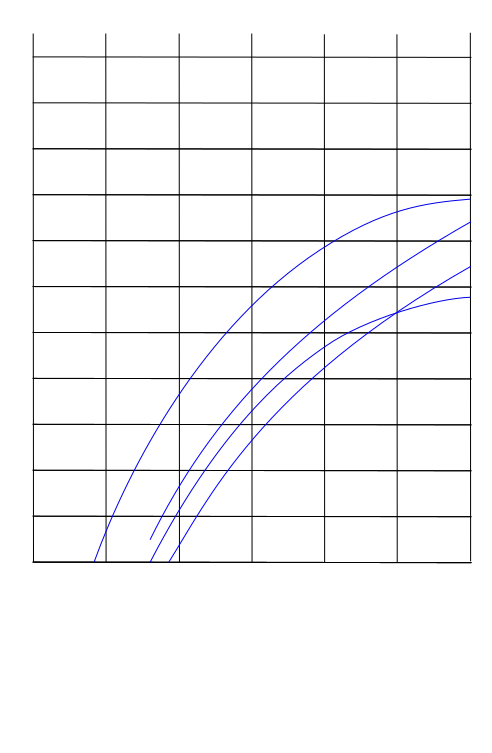
\includegraphics{HeightGraph}
\caption{Ограничения на режимы полета}
\label{fig:ModeOfFlight}
\end{figure}


\begin{figure}[H]
\centering
\def\svgwidth{0.7\textwidth}
\input{figures/BendingMoments.pdf_tex}
\caption{Эпюра изгибающих моментов}
\label{fig:BendingMoments}
\end{figure}

\begin{figure}[H]
\centering
\def\svgwidth{0.7\textwidth}
\input{figures/CuttingForces.pdf_tex}
\caption{Эпюра перерезывающих сил}
\label{fig:CuttingForces}
\end{figure}

\begin{figure}[H]
\centering
\def\svgwidth{0.7\textwidth}
\input{figures/DistributedLoad.pdf_tex}
\caption{Эпюра погонной нагрузки}
\label{fig:DistributedLoad}
\end{figure}

%плавно уточнить, что рассматривать будем в основном изгиб, забив на кручение (рассчеты показывают, что эффект от него небольшой. Возможно, воткнуть график)

